\section{Memorization Examples}
\label{app:memorization}

\begin{figure}[H]
  \centering
  \begin{subfigure}[b]{0.483\textwidth}
    \centering
    \includegraphics[width=\linewidth]{images/repa_imagenette_full_mem.png}
    \caption{Imagenette (memorization)}
  \end{subfigure}
  \hfill
  \begin{subfigure}[b]{0.48\textwidth}
    \centering
    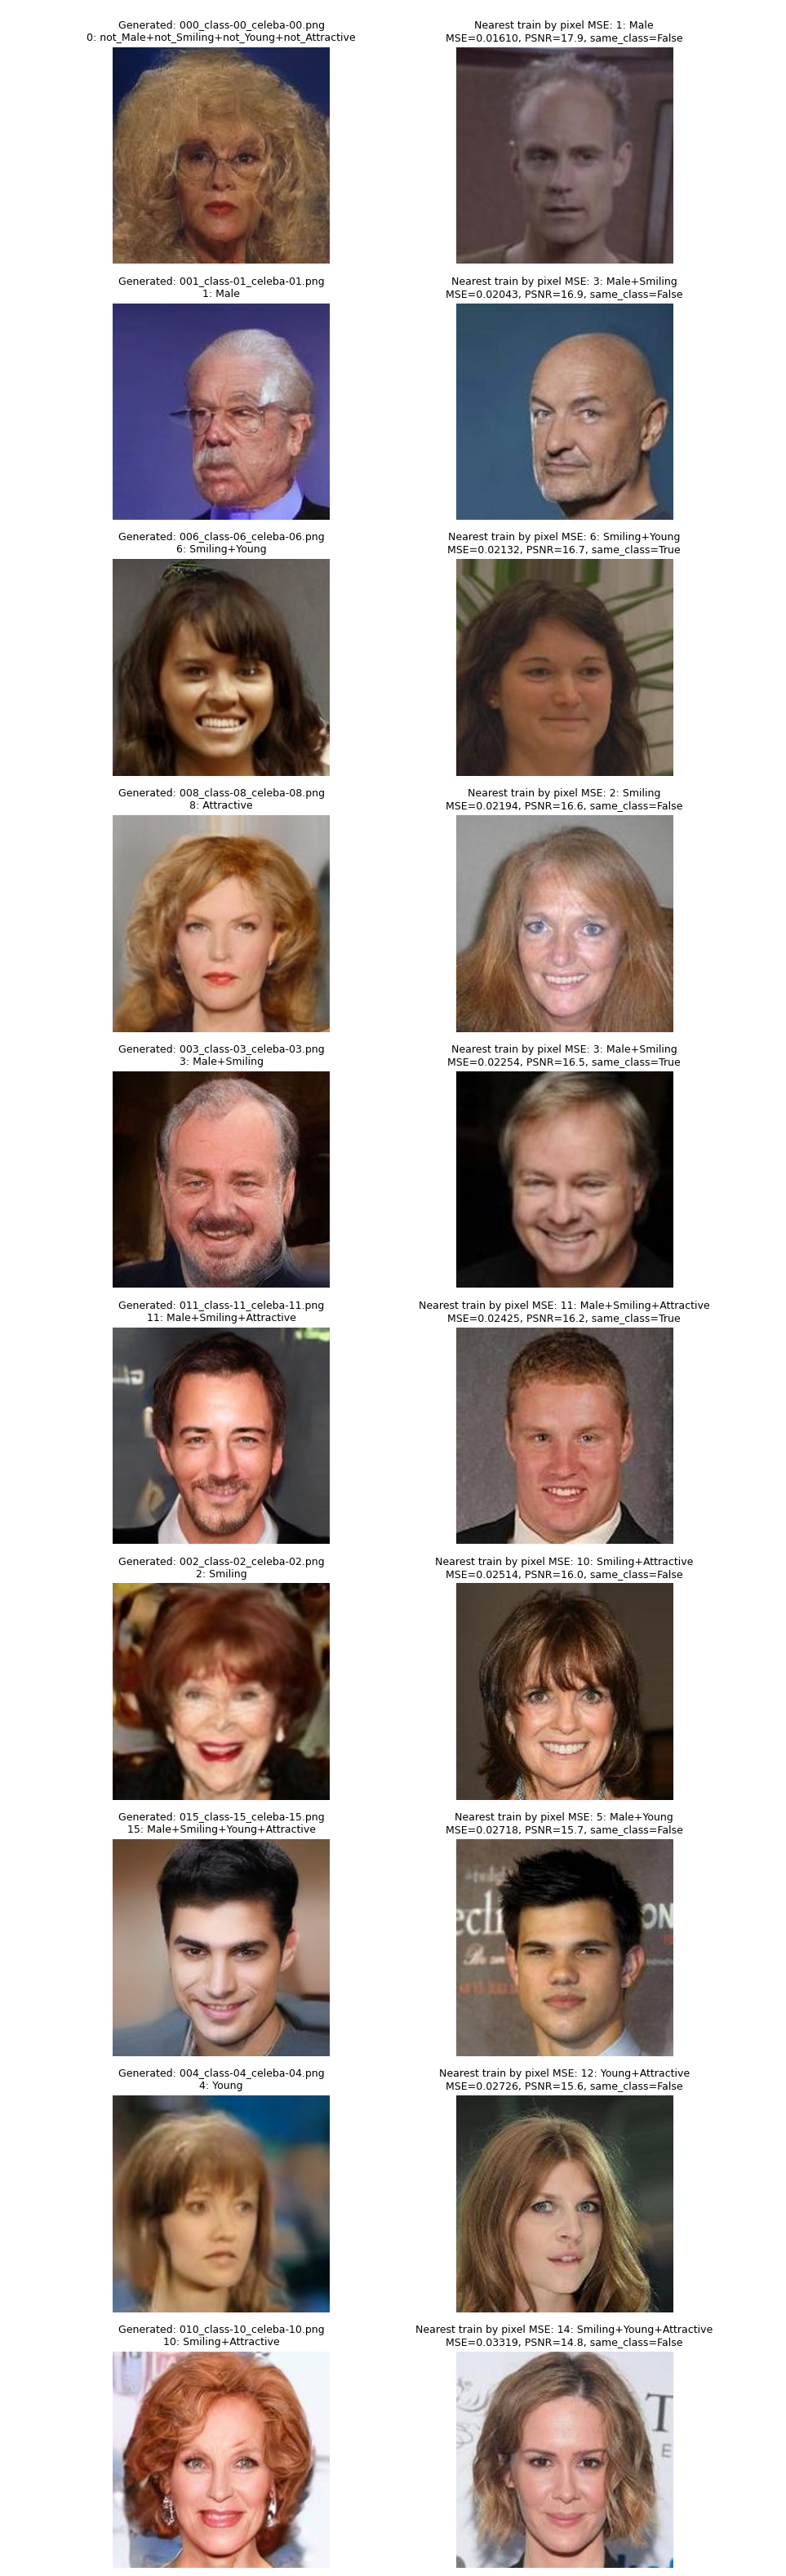
\includegraphics[width=\linewidth]{images/repa_celeba_full_mem.png}
    \caption{CelebA (no memorization)}
  \end{subfigure}
  \caption{Closest dataset images to those generated by diffusion.}
\end{figure}

We first attempted to suppress memorization with an auxiliary batch-variance
diversity loss that penalized low variance across outputs produced from different
noise inputs within a batch. We removed L2 normalization that destroyed the
variance scale and \texttt{.item()} call that detached the loss from the
computation graph. After these fixes the loss collapsed to zero within roughly
100 training steps: the objective is trivially satisfied by high-frequency
colorful noise, which directly conflicts with the structured denoising task.
We therefore abandoned auxiliary diversity regularization and switched to
structural constraints.

\paragraph{Diagnosis of Memorization (Old Model).}

To quantify overfitting, we generate 800 samples (80 per class) from the standard
REPA model (depth 12, no augmentation) after 100k training steps. We use a
classifier-free guidance scale of $w=4.0$, which gives the best perceptual quality
for this model, and evaluate three metrics:
\begin{itemize}
    \item \emph{Nearest-neighbor similarity}: cosine similarity between DINOv2 patch
          features of generated images and the training set. A value close to 1 indicates
          near-exact copying.
    \item \emph{Classification accuracy}: ResNet-50 fine-tuned on ImageNet, evaluated
          on the 10 Imagenette classes (chance level 10\%).
    \item \emph{Diversity}: mean pairwise LPIPS distance over 200 randomly selected
          generations. Higher values indicate more varied outputs.
\end{itemize}

The results, summarised in Table~\ref{tab:imagenette_comparison}, show clear memorization.
The mean similarity of $0.701$ and, more strikingly, $28\%$ of generations have a
training image with similarity $>0.9$ -- a strong indicator of near-copying. The
classification accuracy of $78\%$ is unrealistically high for a generative model
trained on only 10k images; it confirms that the model reproduces training examples
with their original labels. Despite this, diversity remains moderate ($0.689$),
showing that memorization can affect many different training examples without
collapsing to a single mode.

\begin{table}[h]
\centering
\caption{Memorization metrics for the old (depth 12, no augmentation) and new (depth 6, flip augmentation) models at 100k steps, sampled with CFG=4.0.}
\label{tab:imagenette_comparison}
\begin{tabular}{lcccc}
\toprule
Model & Mean similarity & Similarity $>0.9$ & Accuracy & Diversity \\
\midrule
Old (depth 12, no flip) & 0.701 & 28.0\% & 78.0\% & 0.689 \\
New (depth 6, flip)     & 0.470 &  0.0\% & 51.0\% & 0.682 \\
\bottomrule
\end{tabular}
\end{table}

Qualitative evidence supports this diagnosis. Figure~\ref{fig:old_gen} shows ten
randomly selected samples from the old model; although the outputs look plausible at
first glance, many are near-identical copies of training images.
Figure~\ref{fig:old_nn} displays the five most similar pairs (generated image and
its nearest training neighbour), where the visual resemblance is often
indistinguishable.

\begin{figure}
  \centering
  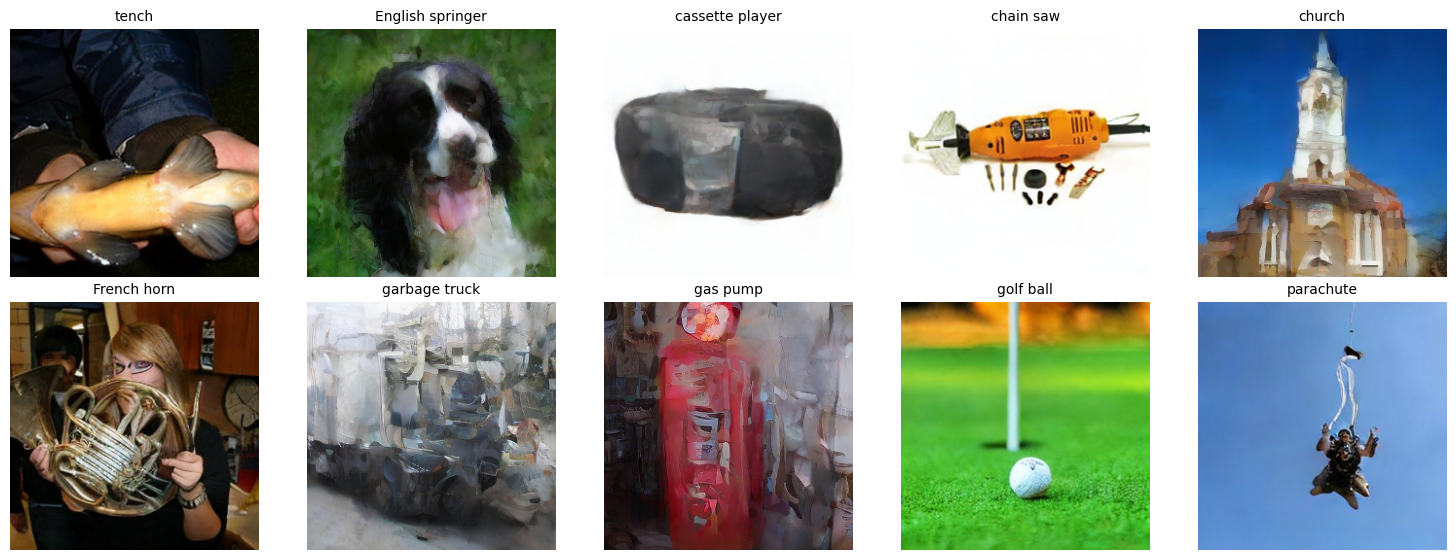
\includegraphics[width=\linewidth]{images/old_model_10_samples.png}
  \caption{Ten random generated images from the old model (depth 12, no augmentation) after 100k steps, CFG=4.0.}
  \label{fig:old_gen}
\end{figure}

\begin{figure}[p]
  \centering
  
\includegraphics[width=\linewidth,height=0.85\textheight,keepaspectratio]{images/old_model_top5_nn.png}
  \caption{Top‑5 most similar pairs (generated image vs. nearest training neighbour) for the old model.}
  \label{fig:old_nn}
\end{figure}
\clearpage

\paragraph{Mitigated Model (Shallow + Flip).}

We repeat the same evaluation for the shallow model trained with random flip
augmentation, after 100k steps and sampled at CFG=4.0. The results are
shown in Table~\ref{tab:imagenette_comparison}. The mean similarity drops to
$0.470$, and crucially, \emph{no} generation has a training neighbour with
similarity $>0.9$ (0.0\%). The classification accuracy falls to a more
reasonable $51\%$ -- still well above chance, indicating that the model has
learned meaningful class distinctions without memorizing specific examples.
Diversity remains virtually unchanged ($0.682$), confirming that the
mitigations do not harm output variety.

Figure~\ref{fig:new_gen} presents ten random samples from the new model. The
images are visually distinct and exhibit greater intra-class variation than
those from the old model. Figure~\ref{fig:new_nn} shows the five most similar
pairs; the nearest training images are now clearly different in pose, lighting,
or fine details -- no exact copies appear.

\begin{figure}[!htb]
  \centering
  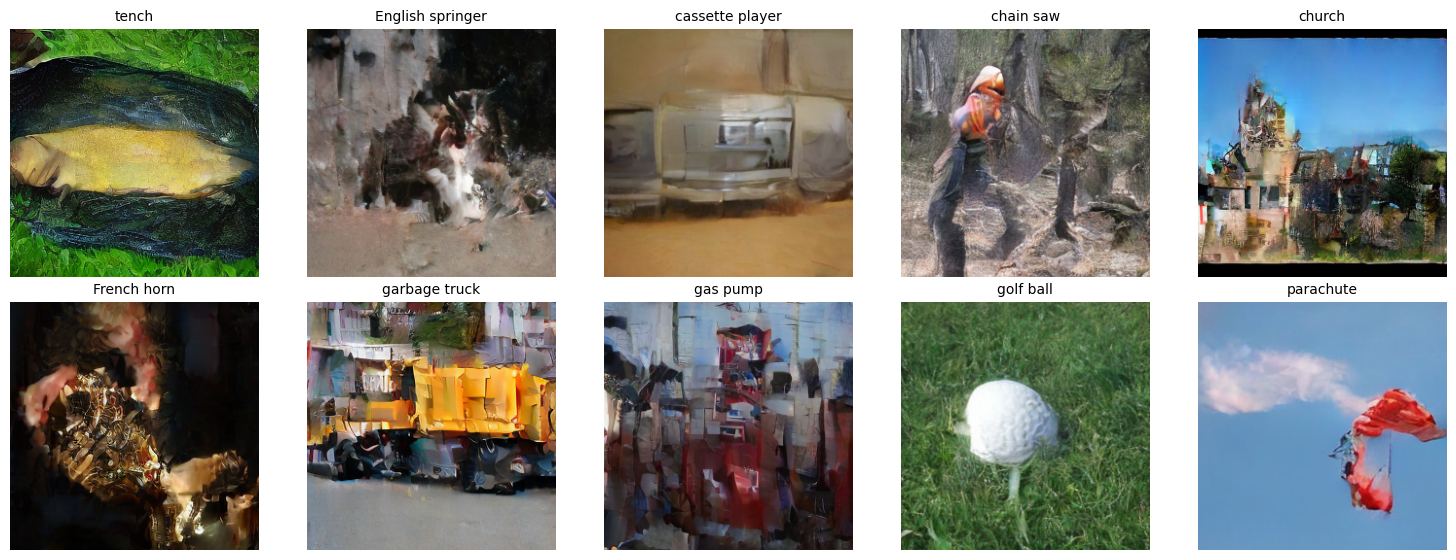
\includegraphics[width=\linewidth]{images/new_model_10_samples.png}
  \caption{Ten random generated images from the new model (depth 6, flip augmentation) after 100k steps, CFG=4.0.}
  \label{fig:new_gen}
\end{figure}

\begin{figure}[p]
  \centering
  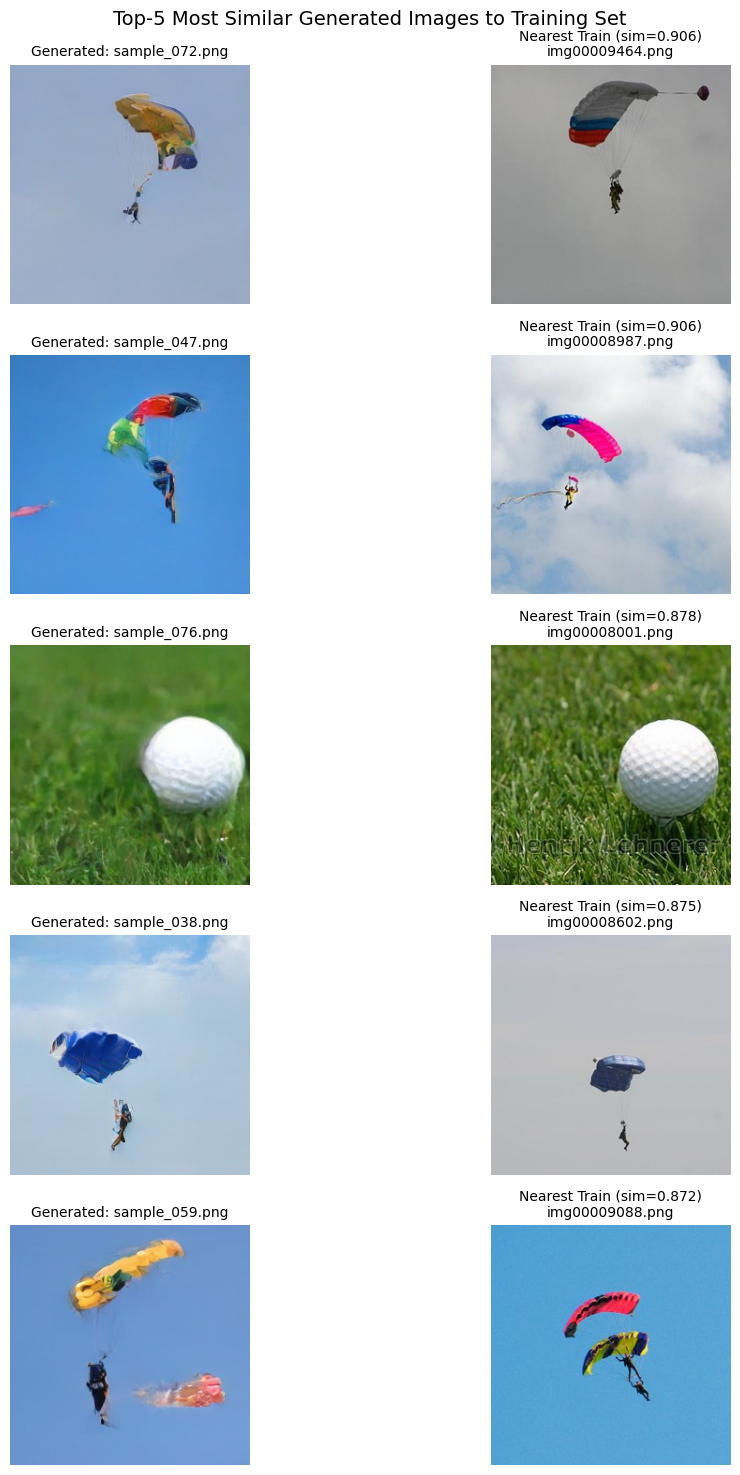
\includegraphics[width=\linewidth,height=0.85\textheight,keepaspectratio]{images/new_model_top5_nn.png}
  \caption{Top‑5 most similar pairs for the new model -- no near‑copies are present.}
  \label{fig:new_nn}
\end{figure}
